\section{Conventional Methods in Action Recognition}
\label{chap:conventional}

This section provides a description of conventional methods in action recognition, i.e.\ methods that do not utilize deep learning techniques and mostly rely on the extraction of hand-crafted features from input-videos.
Due to the availability of several high-quality survey publications in this area, as described in the related work section \ref{sec:relatedwork}, we provide a condensed overview of conventional action recognition methods by describing the main research directions using the taxonomy of \textcite{aggarwal_human_2011}.
For a more detailed description of specific approaches in this area we refer to the publications described in section \ref{sec:relatedwork}.

The approach-based taxonomy of \textcite{aggarwal_human_2011} is depicted in figure \ref{fig:conventional_taxonomy}.
Since its publication in 2011, using space-time features has become the standard approach in video classification \cite{karpathy_large-scale_2014}.
Space-time features are also referred to as local spatio-temporal features, because they describe a local spatio-temporal region of a video.

%We furthermore identify state-of-the art approaches with hand-crafted local features in section \ref{subsec:conventionalsota}.

\begin{figure}[H]
    \centering
    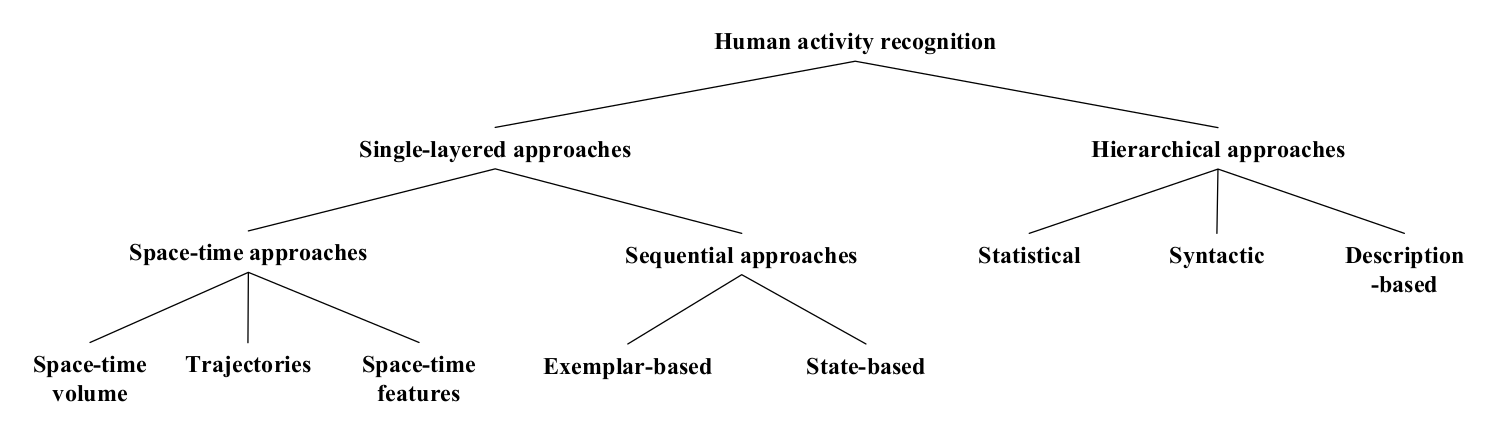
\includegraphics[width=\textwidth]{img_conventional/taxonomy_conventional_methods.png}
    \caption{Approach-based taxonomy for conventional methods in human action recognition as given by Aggarwal and Ryoo \cite{aggarwal_human_2011}}
    \label{fig:conventional_taxonomy}
\end{figure}

\textcite{aggarwal_human_2011} divide the field of activity/action recognition into single-layered and hierarchical approaches.
\begin{description}
    \item[Single-layered Approaches] recognize an action by directly processing raw video-data, i.e.\ based on sequences of video frames.
    \item[Hierarchical Approaches] model an action as a sequence of explicitly defined and individually recognizable atomic sub-actions.
\end{description}

Single-layered approaches are further categorized into space-time approaches and sequential approaches.
\begin{description}
    \item[Space-time approaches] interpret a video as a 3D space-time volume, that results from stacking the individual video-frames along the temporal dimension.
    \item[Sequential approaches] interpret a video as a sequence of observations, i.e.\ feature vectors extracted from individual frames.
\end{description}


\subsection{Single-layered Space-Time Approaches}
Space-time approaches use the entire video volume for action recognition and can be distinguished by what kind of features they use from the volume \cite{aggarwal_human_2011}.
Space-time volume approaches utilize pixel values of the full video volume or parts of it directly for creating a representation of the video, which is then compared with other video volume representations.
Trajectory based approaches use motion trajectories of tracked points inside the volume for the recognition of actions contained in it.
Space-time feature approaches extract features around interest-points locally and aggregate them into a representation of the video volume.


\subsubsection{Action recognition using Space-Time Volumes}
A prototypical approach for action recognition with space-time volumes is described in \cite{aggarwal_human_2011} and uses template matching:
Given a similarity measure for video volumes, the algorithm constructs or selects video volumes template from the training dataset for each action class that has to be recognized.
The template video volumes then act as representations for the action classes.
When presented with a test-video, the algorithm constructs the representation for the new video and compares it to the stored training templates by using the similarity measure.
The action class, that corresponds to the most similar training template is selected as output class for the test-video.

Approaches in this category mainly differ by how a representation is built and how they are compared.
\textcite{bobick_recognition_2001} create templates from the raw video volumes by stacking the silhouettes of persons that perform an action into 2D images.
The resulting binary \textit{motion-energy image} and skalar-valued \textit{motion-history image}, as displayed in figure \ref{fig:spacetimevolumes_meimhi}, are then classified by template matching as described above.

\begin{figure}[h]
    \centering
    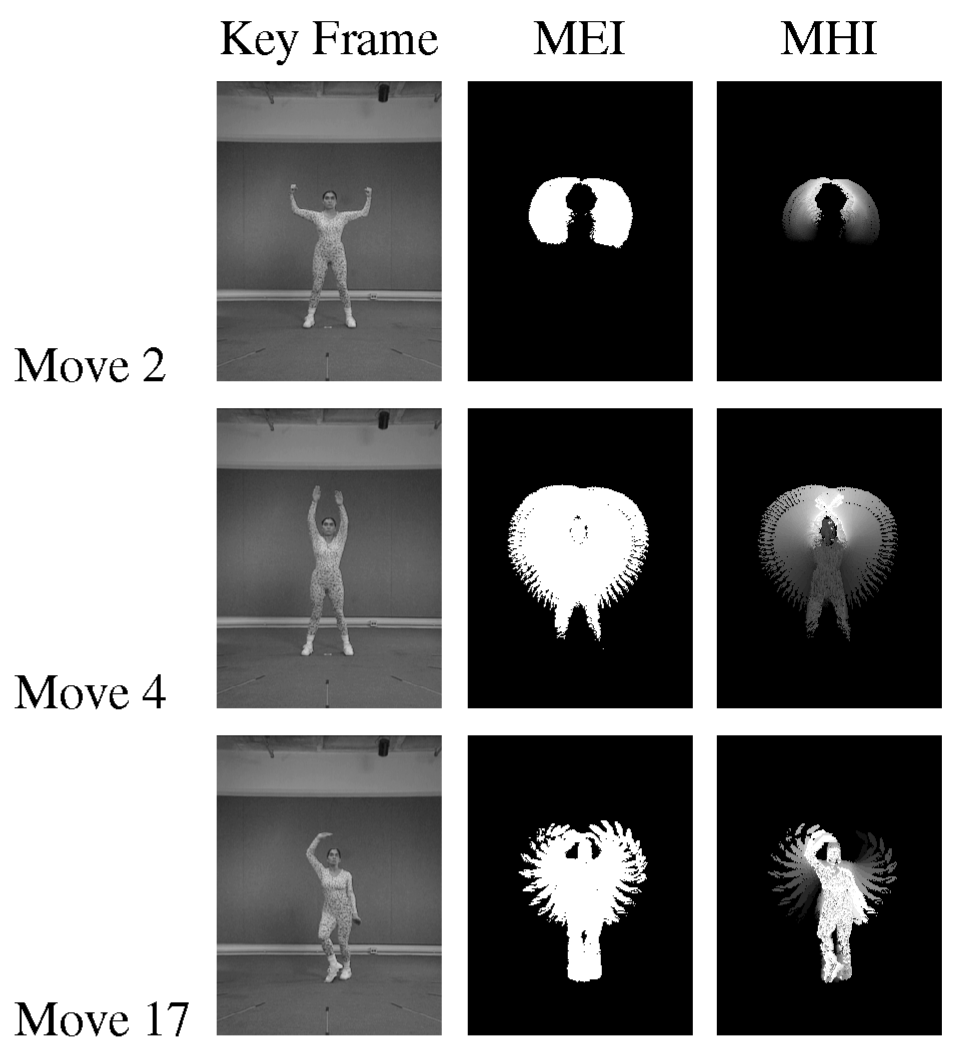
\includegraphics[width=.55\textwidth]{img_conventional/spacetimevolumes_meimhi}
    \caption{Motion-energy image (MEI), motion-history image (MHI) and example frame of three ballet actions \cite{bobick_recognition_2001}}
    \label{fig:spacetimevolumes_meimhi}
\end{figure}


\subsubsection{Action Recognition using Trajectories}
The underlying idea of trajectory-based approaches is, that the motion of a person's joint positions are sufficient for recognizing the performed action \cite{johansson_visual_1975}.
Algorithms that follow this approach use space-time trajectories to represent an action.
More specifically the joint positions of a person are tracked in the video volume.
The resulting trajectories then represent the performed action and can be used for classification, by either comparing the trajectories directly or by extracting features along the trajectories.

\textcite{sheikh_exploring_2005} classify actions by using the trajectories of $13$ tracked points directly as displayed in figure \ref{fig:trajectories_sheikh}.

\begin{figure}[H]
    \centering
    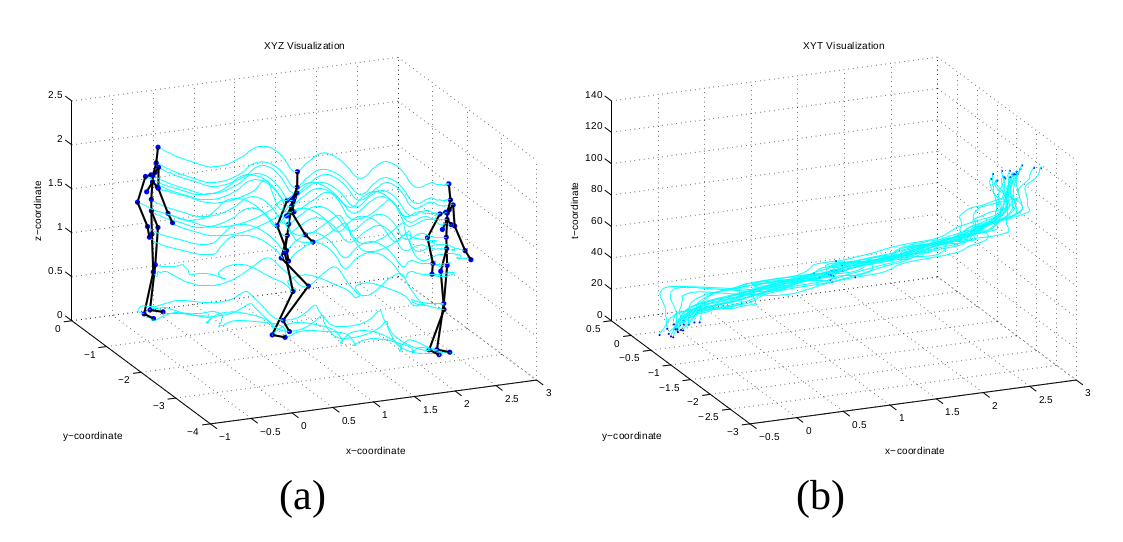
\includegraphics[width=\textwidth]{img_conventional/trajectories_sheikh}
    \caption{Trajectories of a person's tracked joint positions while performing an action. Trajectories shown in XYZ space (a) and XYT space (b) \cite{sheikh_exploring_2005}}
    \label{fig:trajectories_sheikh}
\end{figure}


\subsubsection{Action Recognition using Local Spatio-Temporal Features}
The principle idea behind action recognition with local spatio-temporal features is, that each action produces characteristic changes of pixel values in local 3D regions of the video containing the action \cite{poppe_survey_2010}.
Algorithms can therefore recognize actions by learning the correspondence between an action class and the set of the local regions, that are produced by the class.
A region, that contains these characteristic changes in pixel values, corresponds to a location in the video and is called a \textit{local spatio-temporal feature} or a \textit{spatio-temporal interest point}.
\textcite{aggarwal_human_2011} use the terms interchangeably.

\textcite{poppe_survey_2010} defines spatio-temporal interest points as regions in a video, where sudden changes in motion appear.
They note, that these regions are considered highly informative for action recognition and generally, points that perform a simple translation in the spatio-temporal video volume do not produce a local spatio-temporal feature.

More specifically, \textcite{schuldt_recognizing_2004} define a local space-time feature as ``primitive events corresponding to moving two-dimensional image structures at moments of non-constant motion''.

%In local spatio-temporal feature approaches, a video is generally treated as a 3D space-time volume, which results from stacking the individual video-frames.
%Local regions of characteristic motion are detected in this spatio-temporal volume, which can be interpreted as a three-dimensional object.

In general, a local spatio-temporal feature approach for action recognition contains three main aspects: \cite{karpathy_large-scale_2014}\cite{aggarwal_human_2011}
\begin{enumerate}
    \item \textbf{Feature Extraction}: Determining what kind of features, i.e.\ changes in pixel values, are considered as characteristic for the ongoing motion and where they are located. Feature extractors are specifically hand-crafted to best capture local motion information.
    \item \textbf{Feature Encoding}: Creating a fixed-sized representation of a video using the extracted local spatiotemporal features.
    \item \textbf{Classification}: Learns the correspondence between the video representations and the action class it contains.
\end{enumerate}

Feature extraction can be further divided into interest-point detection and local description \cite{poppe_survey_2010}.
Interest point detectors find and locate the locations of non-constant, informative motion.
Local descriptors transform the raw pixel values in neighbourhoods around previously detected interest points, to best capture the inherent motion information. 

A comparative evaluation of different interest point detectors and local descriptors was published in 2009 by \textcite{wang_evaluation_2009}.
They found, that instead of using computationally expensive feature detectors, dense sampling of interest points from the video is a well performing alternative. 

Prototypical approaches using local features were proposed by \textcite{laptev_space-time_2005} and \textcite{dollar_behavior_2005}.
\textcite{laptev_space-time_2005} extended the Harris corner and edge detector \cite{harris_combined_1988} for extracting space-time interest points in videos.

\begin{figure}[H]
    \centering
    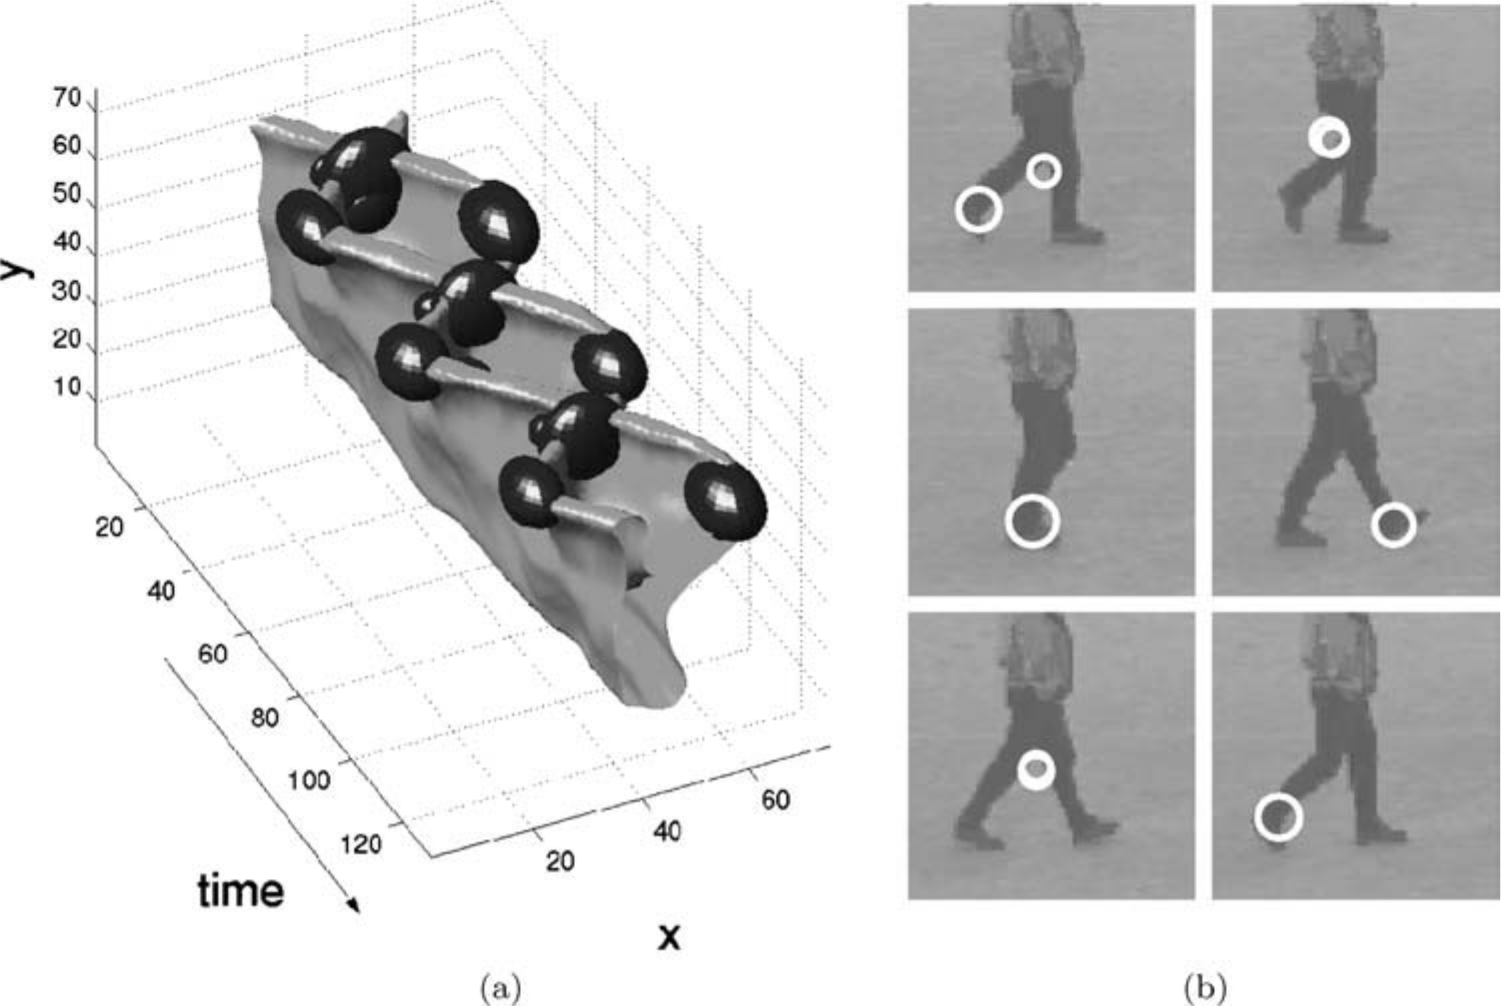
\includegraphics[width=.8\textwidth]{img_conventional/laptev_stip}
\caption{Detection of spatio-temporal interest points from the movement of legs. \textit{a}) Walking pattern of the legs (presented upside down) along with detected interest points (black ellipsoids). \textit{b}) Positions of detected interest points, projected into the original video. \cite{laptev_space-time_2005}}
    \label{fig:laptev_stip}
\end{figure}

\textcite{dollar_behavior_2005} proposed a feature detector for detecting periodic motions.
Once a spatio-temporal interest point is detected, a cube of video pixels called a \textit{Cuboid} as shown in figure \ref{fig:dollar_cuboids} is assigned to each detected point.
The local appearance information in each cube is then extracted and aggregated into a global video description.
They found, that motion information in the cuboids is best captured by transforming each into a flattened vector of brightness gradients to form the final local feature.
Given a training dataset, these final local features in the form of several vectors for each video, are extracted and a codebook of feature vectors is formed by using k-means.
Applying to the bag-of-words paradigm, a video is represented as a histogram of codeword frequencies given the codebook.
Specifically, at first the feature vectors are extracted from a video, each vector is then assigned to its nearest codebook feature vector, which is called a visual word.
By counting the number of visual word occurrences, a histogram representation of the video is created.
A classifier then learns the correlation between histogram representations and action labels.
This approach ignores the spatio-temporal relations between detected interest points.

\begin{figure}[H]
    \centering
    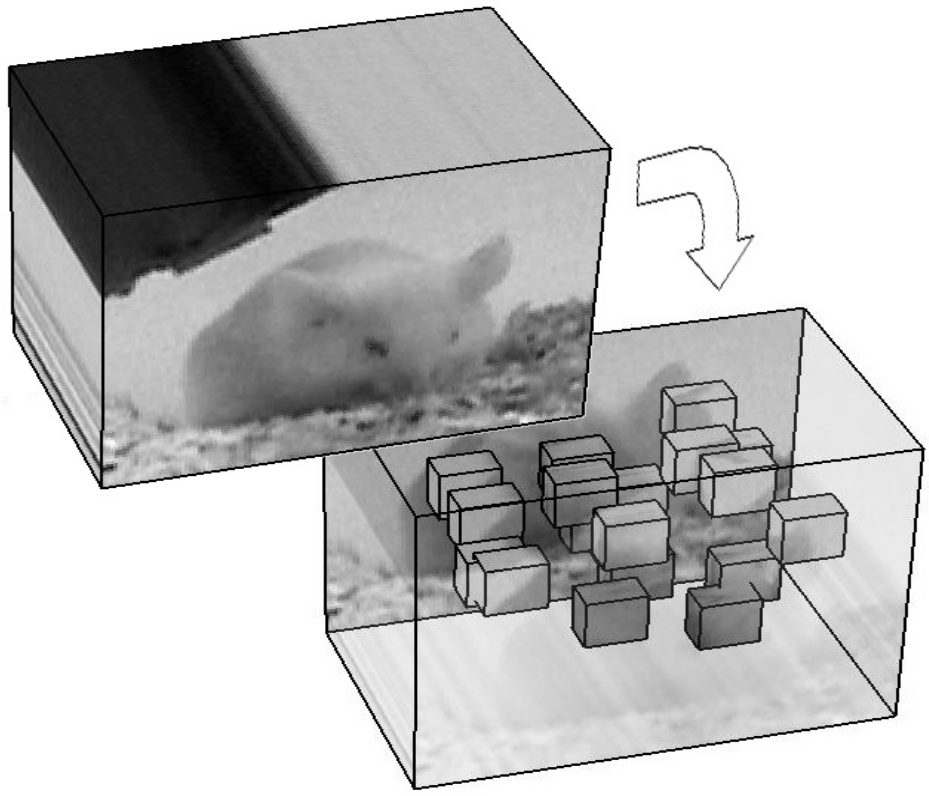
\includegraphics[width=0.4\textwidth]{img_conventional/dollar_cuboids}
    \caption{\cite{dollar_behavior_2005}}
    \label{fig:dollar_cuboids}
\end{figure}

Further examples of feature detectors are given in \cite{poppe_survey_2010}.

Beyond using the bag-of-words paradigm for encoding local features into a global video representation, other more advanced methods were proposed such as the Fisher Vector\cite{perronnin_fisher_2007} and the Vector of Locally Aggregated Descriptors (VLAD) \cite{jegou_aggregating_2010}.
An empirical evaluation of different encoding methods is given in \cite{peng_bag_2014}.

%Laptev and Lindeberg [26] proposed spatio-temporal interest points (STIPs)
%by extending Harris corner detectors to 3D. SIFT and HOG
%are also extended into SIFT-3D [34] and HOG3D [19] for
%action recognition. Dollar et al. proposed Cuboids features
%for behavior recognition [5]. Sadanand and Corso built Ac-
%tionBank for action recognition [33]. Recently, Wang et al.
%proposed improved Dense Trajectories (iDT) [44] which is
%currently the state-of-the-art hand-crafted feature. Tran 2015
%
%Recently, interest point detectors and local descriptors have
%been extended from images to videos. Laptev and Linde-
%berg [13] introduced space-time interest points by extend-
%ing the Harris detector. Other interest point detectors in-
%clude detectors based on Gabor filters [1, 5] or on the de-
%terminant of the spatio-temporal Hessian matrix [33]. Fea-
%ture descriptors range from higher order derivatives (local
%jets), gradient information, optical flow, and brightness in-
%formation [5, 14, 24] to spatio-temporal extensions of image descriptors, such as 3D-SIFT [25], HOG3D [11], extended
%SURF [33], or Local Trinary Patterns [34]. Action Recognition by dense trajectories -- Wang 2011


\subsection{Single-layered Sequential Approaches}
In single-layered sequential approaches an action is processed as a sequence of observations, specifically as a sequence of extracted feature vectors \cite{aggarwal_human_2011}.
As a first step in sequential approaches, feature vectors need to be extracted from each frame in the video that contains the action.
\textcite{aggarwal_human_2011} describe an example of using degrees of joint-angles as suitable feature vectors to describe the status of a person while performing an action.
Given the sequence of feature vectors from in input video, sequential approaches usually calculate the likelihood of action classes producing this observed sequence of feature vectors.
The action class with the highest likelihood is assigned to the input video.

\textcite{aggarwal_human_2011} further differentiate sequential approaches into exemplar-based and state model-based approaches.


\subsubsection{Exemplar-based Approaches}
Exemplar-based approaches store template sequences of feature vectors for each action class \cite{aggarwal_human_2011}:
A presented unknown action in an input video is recognized, by comparing its sequence of feature vectors to the stored templates.
The action class, whose template is most similar to the feature sequence of the input video is assigned to the input.
The approach has to take into account, that the feature sequences may vary because of different execution styles of action among different persons.

The Dynamic Time Warping algorithm (DTW) has been used widely for matching varying sequences in sequential exemplar-based approaches \cite{darrell_space-time_1993}\cite{gavrila_towards_1995}\cite{veeraraghavan_function_2006}.
Following figure \ref{fig:exemplar_dtw} illustrates the concept.

\begin{figure}[H]
    \centering
    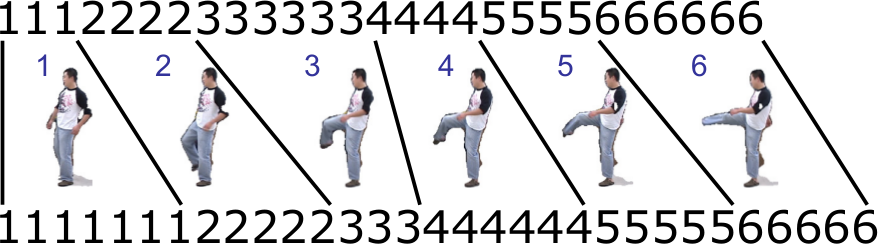
\includegraphics[width=0.6\textwidth]{img_conventional/exemplar_dtw}
    \caption{Matching of two action sequences with different execution rates. Each number corresponds to a pose of the person \cite{aggarwal_human_2011}}
    \label{fig:exemplar_dtw}
\end{figure}

\subsubsection{State Model-based Approaches}
In contrast to representing an action as a sequence of observations, state model-based approaches train one statistical model for each action class and an action is represented as a sequence of the model's hidden states \cite{cheng_advances_2015}.
Using the training videos of an action class, a model is trained on the extracted feature vector observations, so that it generates sequences of feature vectors corresponding to the class.
Given a test video, the likelihood of each model generating this sequence is calculated.
The class, that corresponds to the model with the highest likelihood, is assigned to the test video.
Hidden Markov Models and Dynamic Bayesian Networks have been used for these approaches \cite{aggarwal_human_2011}.


\subsection{Hierarchical Approaches}
The main idea of hierarchical approaches is to model complex actions as a hierarchy of simpler sub-actions \cite{aggarwal_human_2011}.
Sub-actions themselves can be further decomposed, until the initial complex action is represented as a sequence of non-decomposable atomic sub-actions.
A complex action is interpreted as a process that generates sub-actions which can be observed and classified individually.
Most hierarchical approaches thereby employ non-hierarchical single-layered action recognition approaches to recognize low-level sub-actions.

\textcite{aggarwal_human_2011} further differentiate hierarchical approaches into statistical approaches, syntactic approaches and desciption-based approaches.


\subsubsection{Statistical Approaches} 
Hierarchical statistical approaches use hierarchically stacked state-based models such as Hidden Markov Models (HMMs) \cite{oliver_layered_2002}\cite{zhang_modeling_2004} or Dynamic Bayesian Networks (DBNs) \cite{dai_group_2008}\cite{gong_recognition_2003} for action recognition.
Typically two layers of such models are used, where the bottom layer recognizes simple actions from sequences of feature vectors and the top layer recognizes high-level actions from the resulting sequence of simple actions.
The layered Hidden Markov Model approach of \textcite{oliver_layered_2002} is said to be one of the most fundamental forms of hierarchical statistical approaches \cite{aggarwal_human_2011}.


\subsubsection{Syntactic Approaches} 
In hierarchical syntactic approaches, a high-level action is represented as a string of symbols \cite{cheng_advances_2015}.
Each symbol therein corresponds to a simpler, possibly atomic, sub-action as described previously.
Equivalently to hierarchical statistical approaches, syntactic approaches require the recognition of sub-actions by using any of the previously described methods in order to obtain the string of symbols.
An action class is represented as a set of production rules from context-free grammars or stochastic context-free grammars \cite{ivanov_recognition_2000}\cite{moore_recognizing_2002}\cite{minnen_expectation_2003}\cite{joo_attribute_2006}, that generate sequences of symbols corresponding to the action class.
Syntactic approaches then use parsing techniques from the field of programming languages \cite{hopcroft_introduction_1979} to recognize high-level actions.


\subsubsection{Description-based Approaches}
The definition of description-based approaches by \textcite{aggarwal_human_2011} states: ``A description-based approach is a recognition approach, that explicitly maintains human activities' spatio-temporal structure.''
High-level actions are represented by occurrences of their underlying sub-actions, while temporal, spatial and logical relationships between the sub-actions are explicitly specified.
The temporal relations between sub-actions are usually specified by associating a time interval with an occurring action.
\textcite{allen_maintaining_1983}\cite{allen_actions_1994} introduced seven predicates to describe temporal relations between time intervals: \textit{before, meets, overlaps, during, starts, finishes} and \textit{equals}, which have been widely used for hierarchical description-based approaches \cite{pinhanez_human_1998}\cite{siskind_grounding_2001}\cite{nevatia_hierarchical_2003}\cite{ryoo_recognition_2006}.


\subsection{State of the Art Approaches using Local Features}
\label{subsec:conventionalsota}

\textcite{wang_action_2013} introduced the \textit{Improved Dense Trajectories} approach, which is often considered state of the art in action recognition using hand-crafted local features \cite{tran_learning_2015}\cite{wang_towards_2015}\cite{simonyan_two-stream_2014}.
Using the categorization proposed by the taxonomy of \textcite{aggarwal_human_2011}, it can be seen as a hybrid approach of being trajectory-based and using hand-crafted local features.The principle idea behind \textit{Improved Dense Trajectories} is to densely sample spatio-temporal interest points, tracking them using optical flow and extracting local hand-crafted features in regions around the resulting point trajectories.

A basic version of the approach, called \textit{Dense Trajectories}, was first published in 2011 \cite{wang_action_2011} and later improved in 2013 (\textit{Improved Dense Trajectories}) \cite{wang_action_2013}.

A comparison of hand-crafted feature approaches to recent deep learning methods in action recognition is given in section \ref{sec:evaluation}.
Beyond \textit{Improved Dense Trajectories}, the following approaches have been considered state of the art \cite{wang_towards_2015}\cite{lan_beyond_2015}and are compared as well:
\begin{itemize}
    \item Multi-view super vector for action recognition (2014) \cite{cai_multi-view_2014}
    \item Beyond Gaussian pyramid: Multi-skip feature stacking for action recognition (2015) \cite{lan_beyond_2015}
\end{itemize}

\subsubsection{Action Recognition by Dense Trajectories (2011)}
\textcite{wang_action_2011} introduce a tracking technique called \textit{dense trajectories} for action classification from videos.
Points are sampled densely from each frame and then tracked using a dense optical flow field.
Local spatio-temporal features are extracted in regions around the resulting point trajectories to form trajectory descriptors, which are then aggregated into a global video descriptor using the bag-of-words paradigm.

%
%Dense sampling of interest points has shown to yield improved performance in action recognition over sparse spatio-temporal interest points \cite{wang_evaluation_2009}.
%However using the KLT tracker to obtain dense trajectories or matching SIFT features on densely sampled points would be computationally too expensive to handle large datasets. 
%The authors approach therefore represents an efficient way to extract dense trajectories.

Since motion in a video, and therefore also the resulting trajectories, can stem from either motion of interest or unwanted camera motion, the authors propose using a descriptor called \textit{Motion Boundary Histogram} (MBH), which aims at focussing on foreground motion.
The MBH descriptor is designed to make the classification of actions in a video invariant to camera motion.

The overall approach for obtaining a descriptor along densely extracted trajectories is shown in figure \ref{fig:densetrajectories_approach}

\begin{figure}[H]
    \centering
    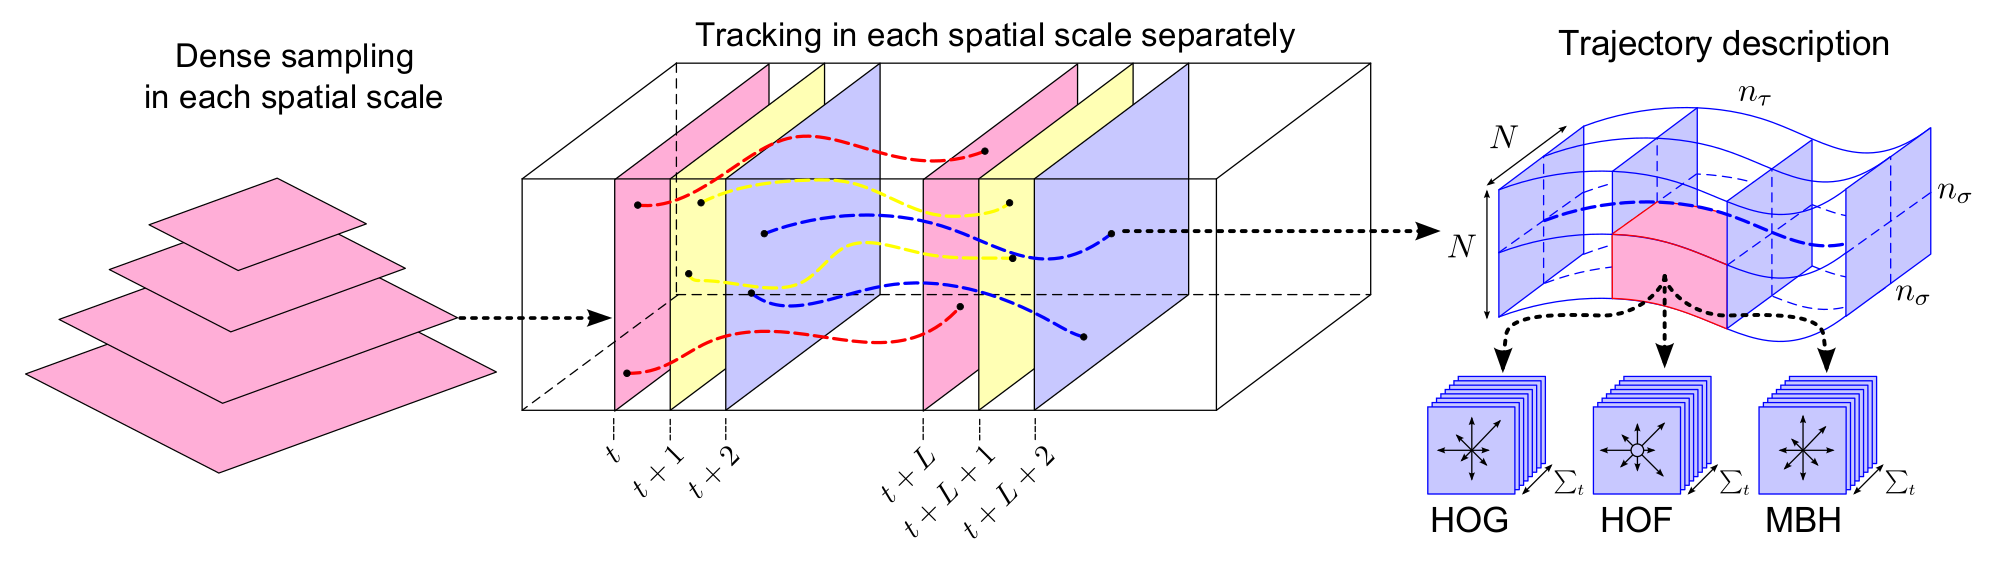
\includegraphics[width=\textwidth]{img_conventional/densetrajectories_approach}
    \caption{Description of densely extracted trajectories \cite{wang_action_2011}}
    \label{fig:densetrajectories_approach}
\end{figure}

Dense trajectories are obtained separately from 8 spatial scales, which differ by a factor of $1 / \sqrt{2}$.
Points are sampled on a grid spaced by $W$ pixels on each scale. Experimentally $W = 5$ has been shown to yield good results.
Each point $P_t$ at frame $t$ is tracked to the next frame by using a dense optical flow field, which was extracted by the Farnebäck algorithm \cite{farneback_two-frame_2003} as implemented in OpenCV.
%The tracked points in subsequent frames then form the trajectory $(P_t, P_{t+1}, P_{t+2}, \cdots)$.
%The maximum length of a trajectory is limited to $L = 15$ frames to avoid the problem of drifting.
%Trajectories that exceed this limit are removed from the tracking process.
%The presence of a trackectory in each $W \times W$ unit of each frame is verified. If no tajectory is present, a new point is sampled and added to the tracking process.

Since only dynamic information is important for action recognition, static trajectories are removed in a pre-processing stage.
Erroneous trajectories with sudden large displacements are also removed.

A simple descriptor is obtained from the shape of a trajectory itself.
It is formed by normalizing the spatial displacements given by the differences of consecutive points in a trajectory.
Formally the \textit{trajectory descriptor} $S'$ is given by:
\begin{equation*}
    S' = \frac{(\Delta P_t, \cdots, \Delta P_{t+L-1})}{\sum_{j=t}^{t+L-1} \|P_j\|}
\end{equation*}
Where $\Delta P_t = (P_{t+1} - P_t) = (x_{t+1} - x_t, y_{t+1} - y_t)$.

\textbf{Local Feature Descriptors:}\\
Local features are extracted from video volumes of size $N \times N \times L$ around the trajectories as depicted in figure \ref{fig:densetrajectories_approach}, where $N = 32$ has shown to yield good results.

Feature descriptors evaluated in the context of dense trajectories are):
\begin{itemize}
    \item \textbf{HOG} (Histogram of Oriented Gradients) \cite{dalal_histograms_2005-1}
    \item \textbf{HOF} (Histogram of Optical Flow) \cite{laptev_learning_2008}
    \item \textbf{MBH} (Motion Boundary Histogram) \cite{dalal_human_2006}
\end{itemize}

\begin{figure}[H]
    \centering
    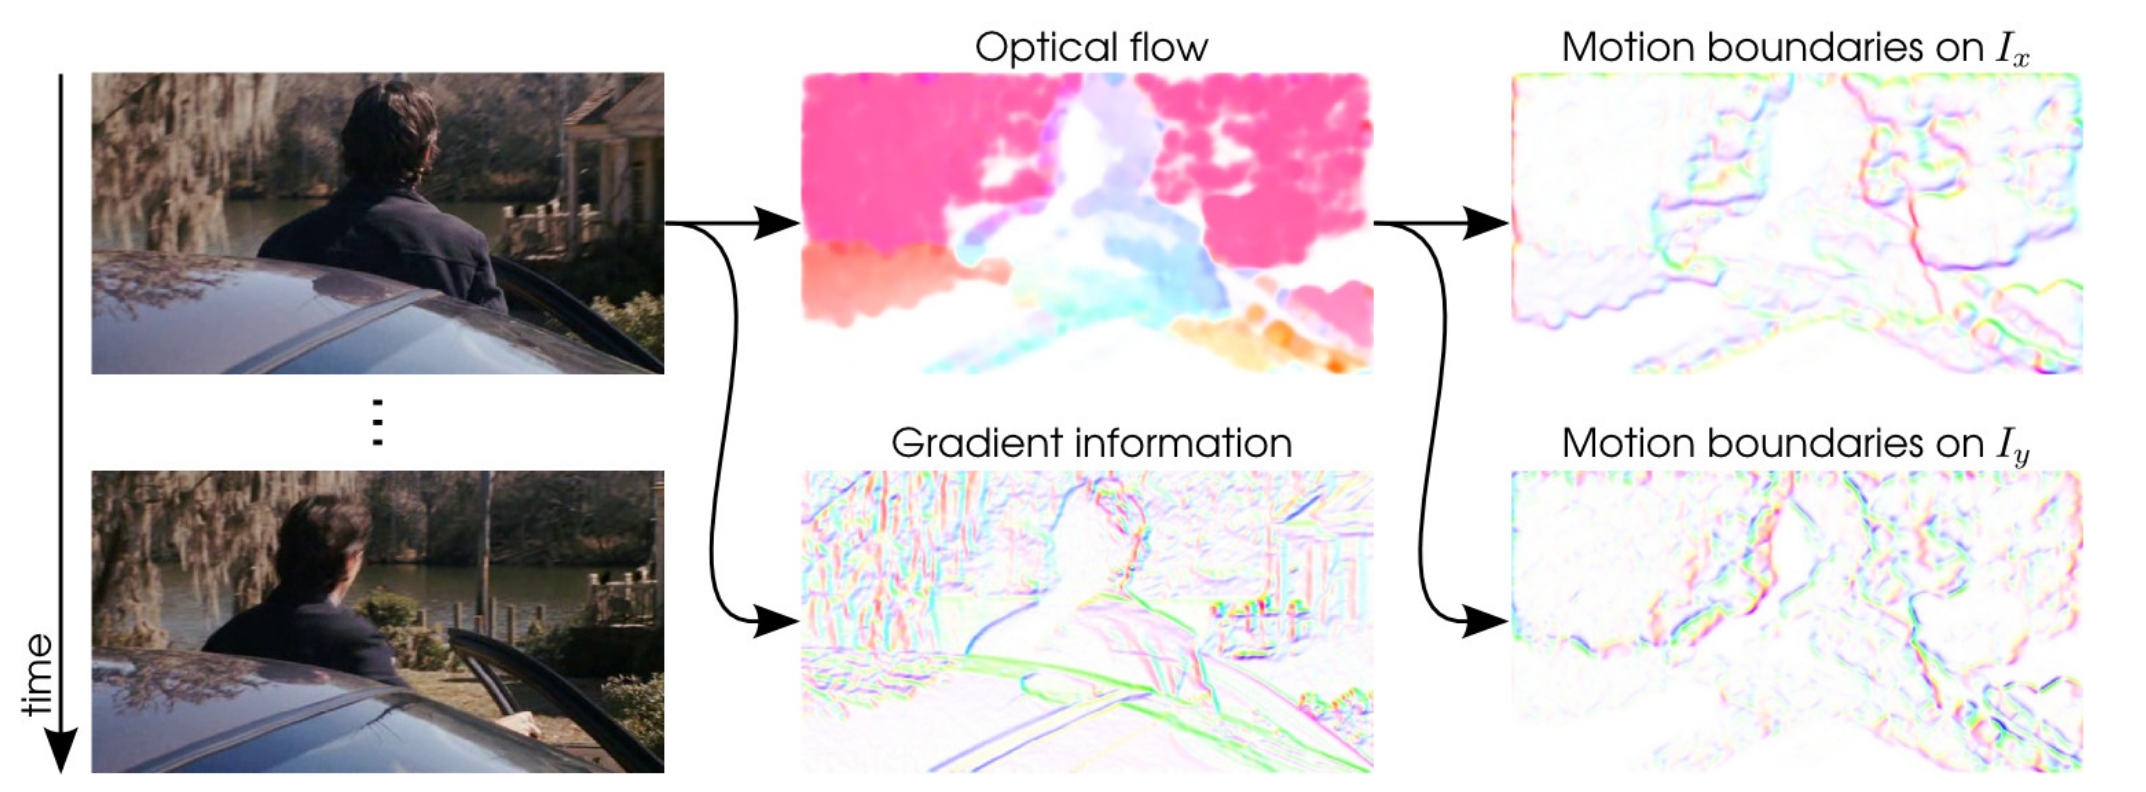
\includegraphics[width=\textwidth]{img_conventional/densetrajectories_featurevisualization}
    \caption{Visualization of the information captured by HOG, HOF and MBH on complete video frames. In each image, the orientation is given by color, the magnitude is given by saturation. \cite{wang_action_2011}}
    \label{fig:densetrajectories_featurevisualization}
\end{figure}

The HOG descriptor encodes static appearance information by computing the orientations of image gradients and aggregating them in a histogram over all subframes of the current video volume along the trajectory. In this approach the histograms contain 8 bins.

The HOF descriptor aggregates the orientations of optical flow vectors in a histogram and therefore captures local motion information. An additional bin is used here.

The MBH descriptor separately calculates the spatial derivatives of the $x$- and $y$-component of the optical flow field.
The orientations of the derivatives are aggregated into histograms (similarly to the HOG descriptor), which represent the video volume.
An advantage of MBH is that is suppresses constant motion, since it takes only the changes in the flow field (i.e.\ motion boundaries) into account.
The authors therefore use MBH as an easy way to filter noise stemming from background camera-motion, as can be seen by comparing the optical flow-image and motion boundaries in figure \ref{fig:densetrajectories_featurevisualization}.

The authors evaluate their approach on the KTH, YouTube, Hollywood2 and UCF-Sports dataset using a standard bag-of-features approach as follows:

\begin{enumerate}
    \item Construction of a codebook for each descriptor-type (trajectory, HOG, HOF and MBH).
        $100.000$ descriptors for each type are randomly chosen from all extracted descriptors over the training split.
        These descriptors are clustered into a 4000 words long codebook using $k$-means.
    \item Each extracted descriptor from a video is assigned to its nearest codebook-descriptor using the Euclidean distance.
        The number of occurrences are aggregated in a histogram, which builds the global video descriptor.
    \item A classifier (here a non-linear SVM with a $\chi^2$ kernel) is trained to assign the class-labels to the global video descriptors.
\end{enumerate}

Besides densely sampled trajectories, the authors evaluate baseline trajectories obtained from the KLT tracker for comparison.
The same descriptors (trajectory, HOG, HOF and MBH) are used around the KLT-trajectories.

\begin{table}[H]
    \centering
    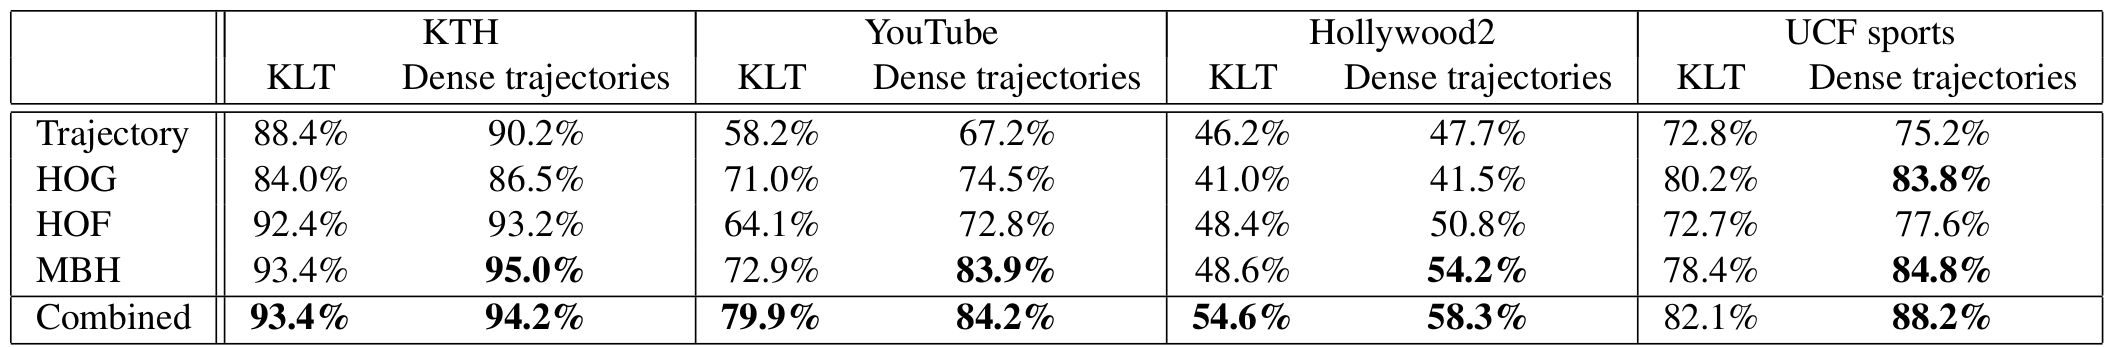
\includegraphics[width=\textwidth]{img_conventional/densetrajectories_results}
    \caption{Results of dense trajectories compared to KLT-trajectories when using different feature descriptors. \cite{wang_action_2011}}
    \label{tab:densetrajectories_results}
\end{table}

Other approaches used feature trajectories for action recognition by either tracking sparse spatio-temporal interest points using a standard KLT tracker \cite{lucas_iterative_1981} or by matching SIFT features \cite{lowe_distinctive_2004} between consecutive frames.
The results in table \ref{tab:densetrajectories_results} show the superiority of dense trajectories compared to the KLT baseline.
The simple trajectory descriptor yields surprisingly good results, which according to the authors confirms the importance of motion information encoded in the trajectory shapes themselves.
The MBH descriptor performs significantly better than all the other descriptors.
On the YouTube dataset, the advantage of using the MBH descriptor is most prominent, since the videos in this dataset contain a lot of noise from camera-motion (uncontrolled, realistic videos, often recorded by handheld cameras).


\subsubsection{Action recognition with improved trajectories (2013)}
\textcite{wang_action_2013} address a problem of their previously released \textit{Dense Trajectories} approach.
Sampling of interest points and tracking them to from trajectories uses optical flow fields between frames.
Motion that results from camera movement however, also produces optical flow in the background of an image, which results in trajectories that do not convey relevant information about the ongoing action in the scene.

\textcite{wang_action_2013} address this problem by explicitly estimating a homography between two frames, to compensate camera motion. 
Results of the approach are illustrated in figure \ref{fig:trajectories_improved}.

\begin{figure}[H]
    \centering
    \includegraphics[width=0.6\textwidth]{img_conventional/trajectories_improved}
    \caption{Improved dense trajectories: First row shows two overlaid consecutive frames, second row shows the resulting optical flow (notice the background), third row shows the optical flow after removing camera motion, fourth row shows trajectories that were removed due to camera motion estimation (white). \cite{wang_action_2013}}
    \label{fig:trajectories_improved}
\end{figure}

Camera motion estimation was able to further improve the performance of dense trajectories, resulting in the approach being considered state of the art \cite{tran_learning_2015}.
